\HC[All]{Maybe one section of each of these}

\subsection{Prototype evaluation}

\begin{itemize}
%\item description of synthetic benchmarks
\item experimental setup
\item results and comments
\end{itemize}
This section evaluates the performance of Madeus with empty transitions.
Madeus is a model that relies on the description of an \emph{internal-net} (life-cycle) for each component of the software that will be deployed. It is a low-level model, therefore the developer is responsible for the choices of actions performed in the transitions.

The aim is to evaluate Madeus independently of any specific transitions which is why these experiments are called \emph{dry-runs}. It means the transitions do not contain any action which allows to measure the overhead caused by Madeus.

% figures to add for assemblies
%Sequential

\begin{figure}[h]
  \begin{center}
    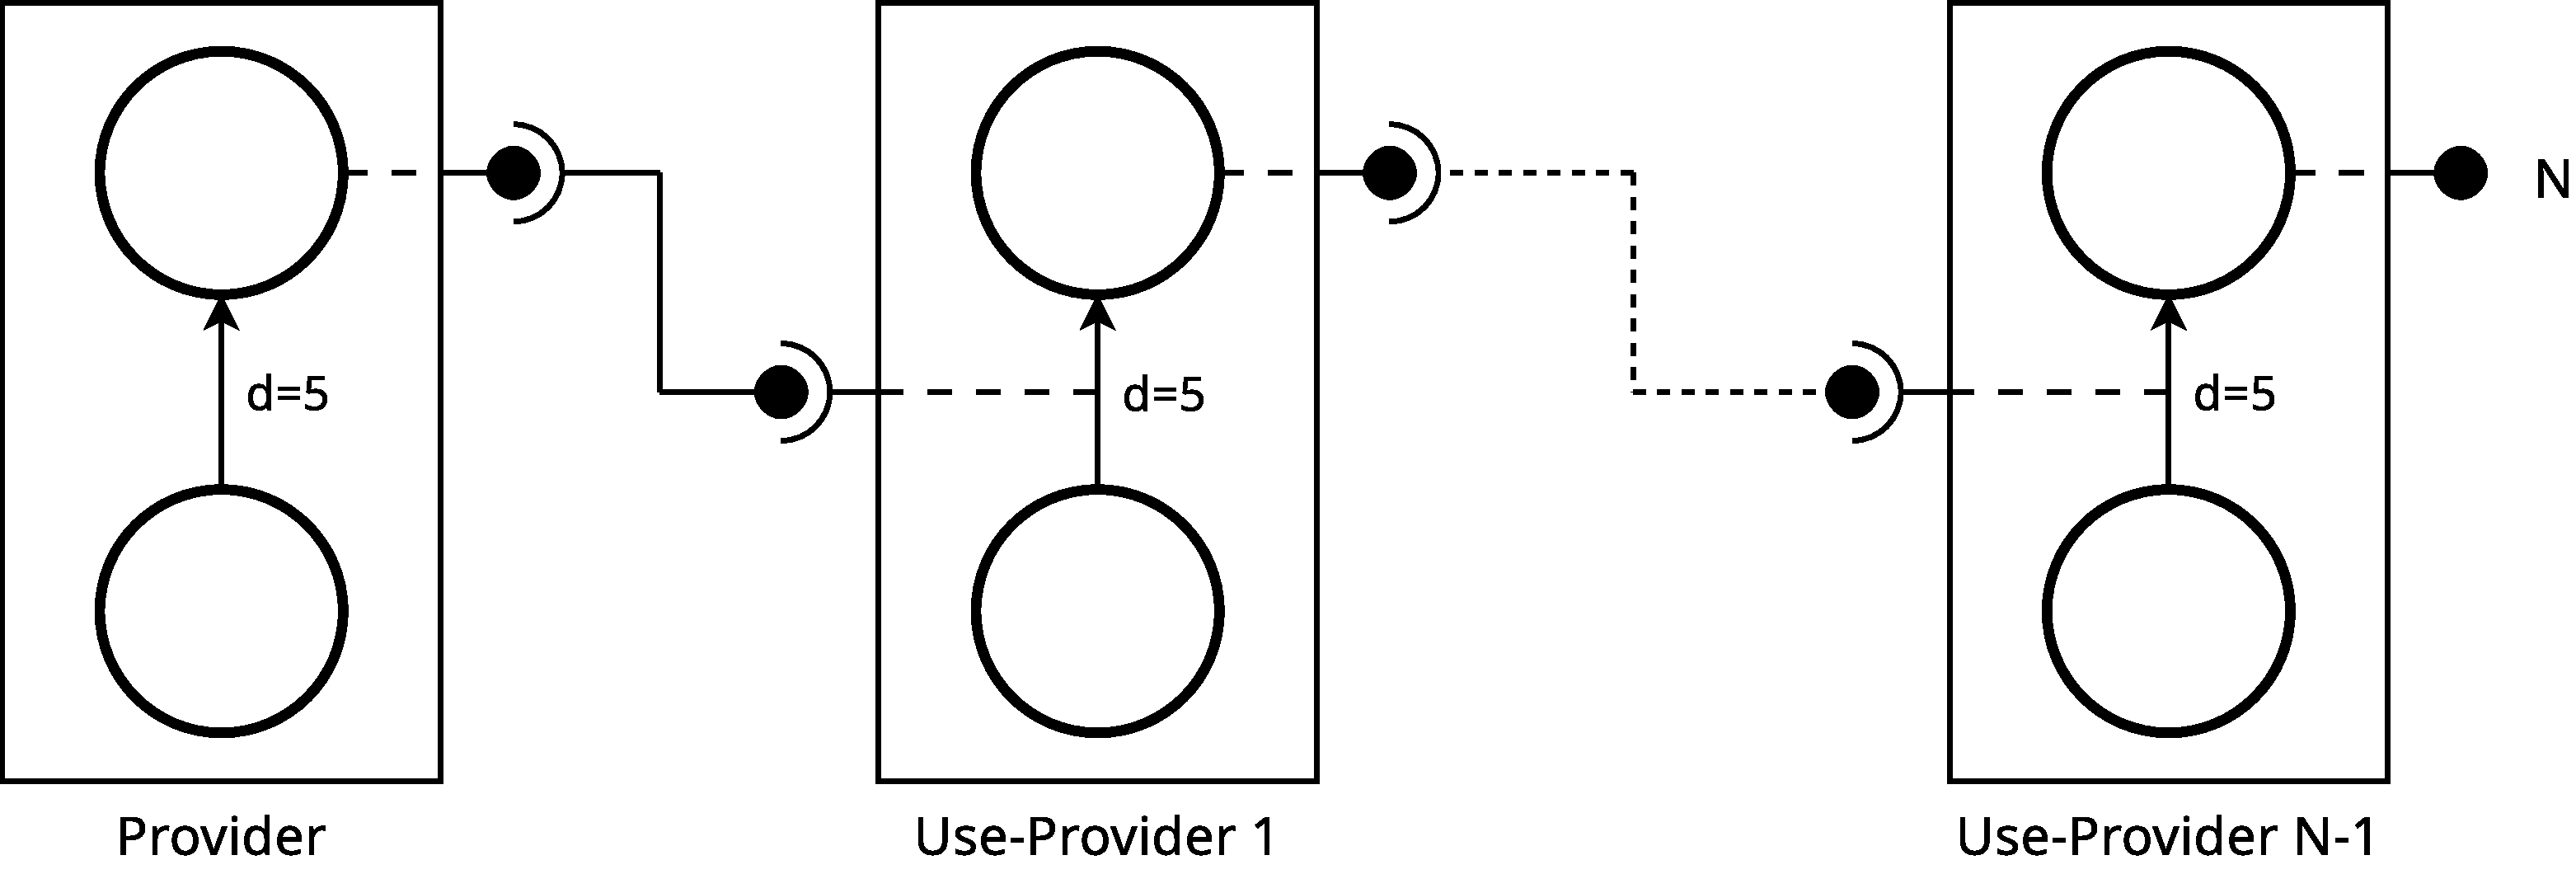
\includegraphics[width=0.4\textwidth]{./images/seq.pdf}
    \caption{The sequential assembly for the Madeus benchmark, with N components.}
    \label{fig:seq}
  \end{center}
\end{figure}

Three benchmarks are the base of this evaluation. The first benchmark is made with a sequential assembly written in Madeus, depicted in Figure~\ref{fig:seq}
and made of a chain of components: one \emph{provider} component made of a transition and two places, the final one providing a service, and \emph{N user-provider} components that are also composed of a transition and two places, but where the transition uses the provide port of the preceeding component. The components are connected and this results in a sequential execution.

A dry-run version of this assembly is built containing transitions that do nothing besides wait for a fixed amount of time. As it is a sequential assembly, the execution time should be increasing with the number of \emph{N} components.

\begin{figure}[h]
  \begin{center}
    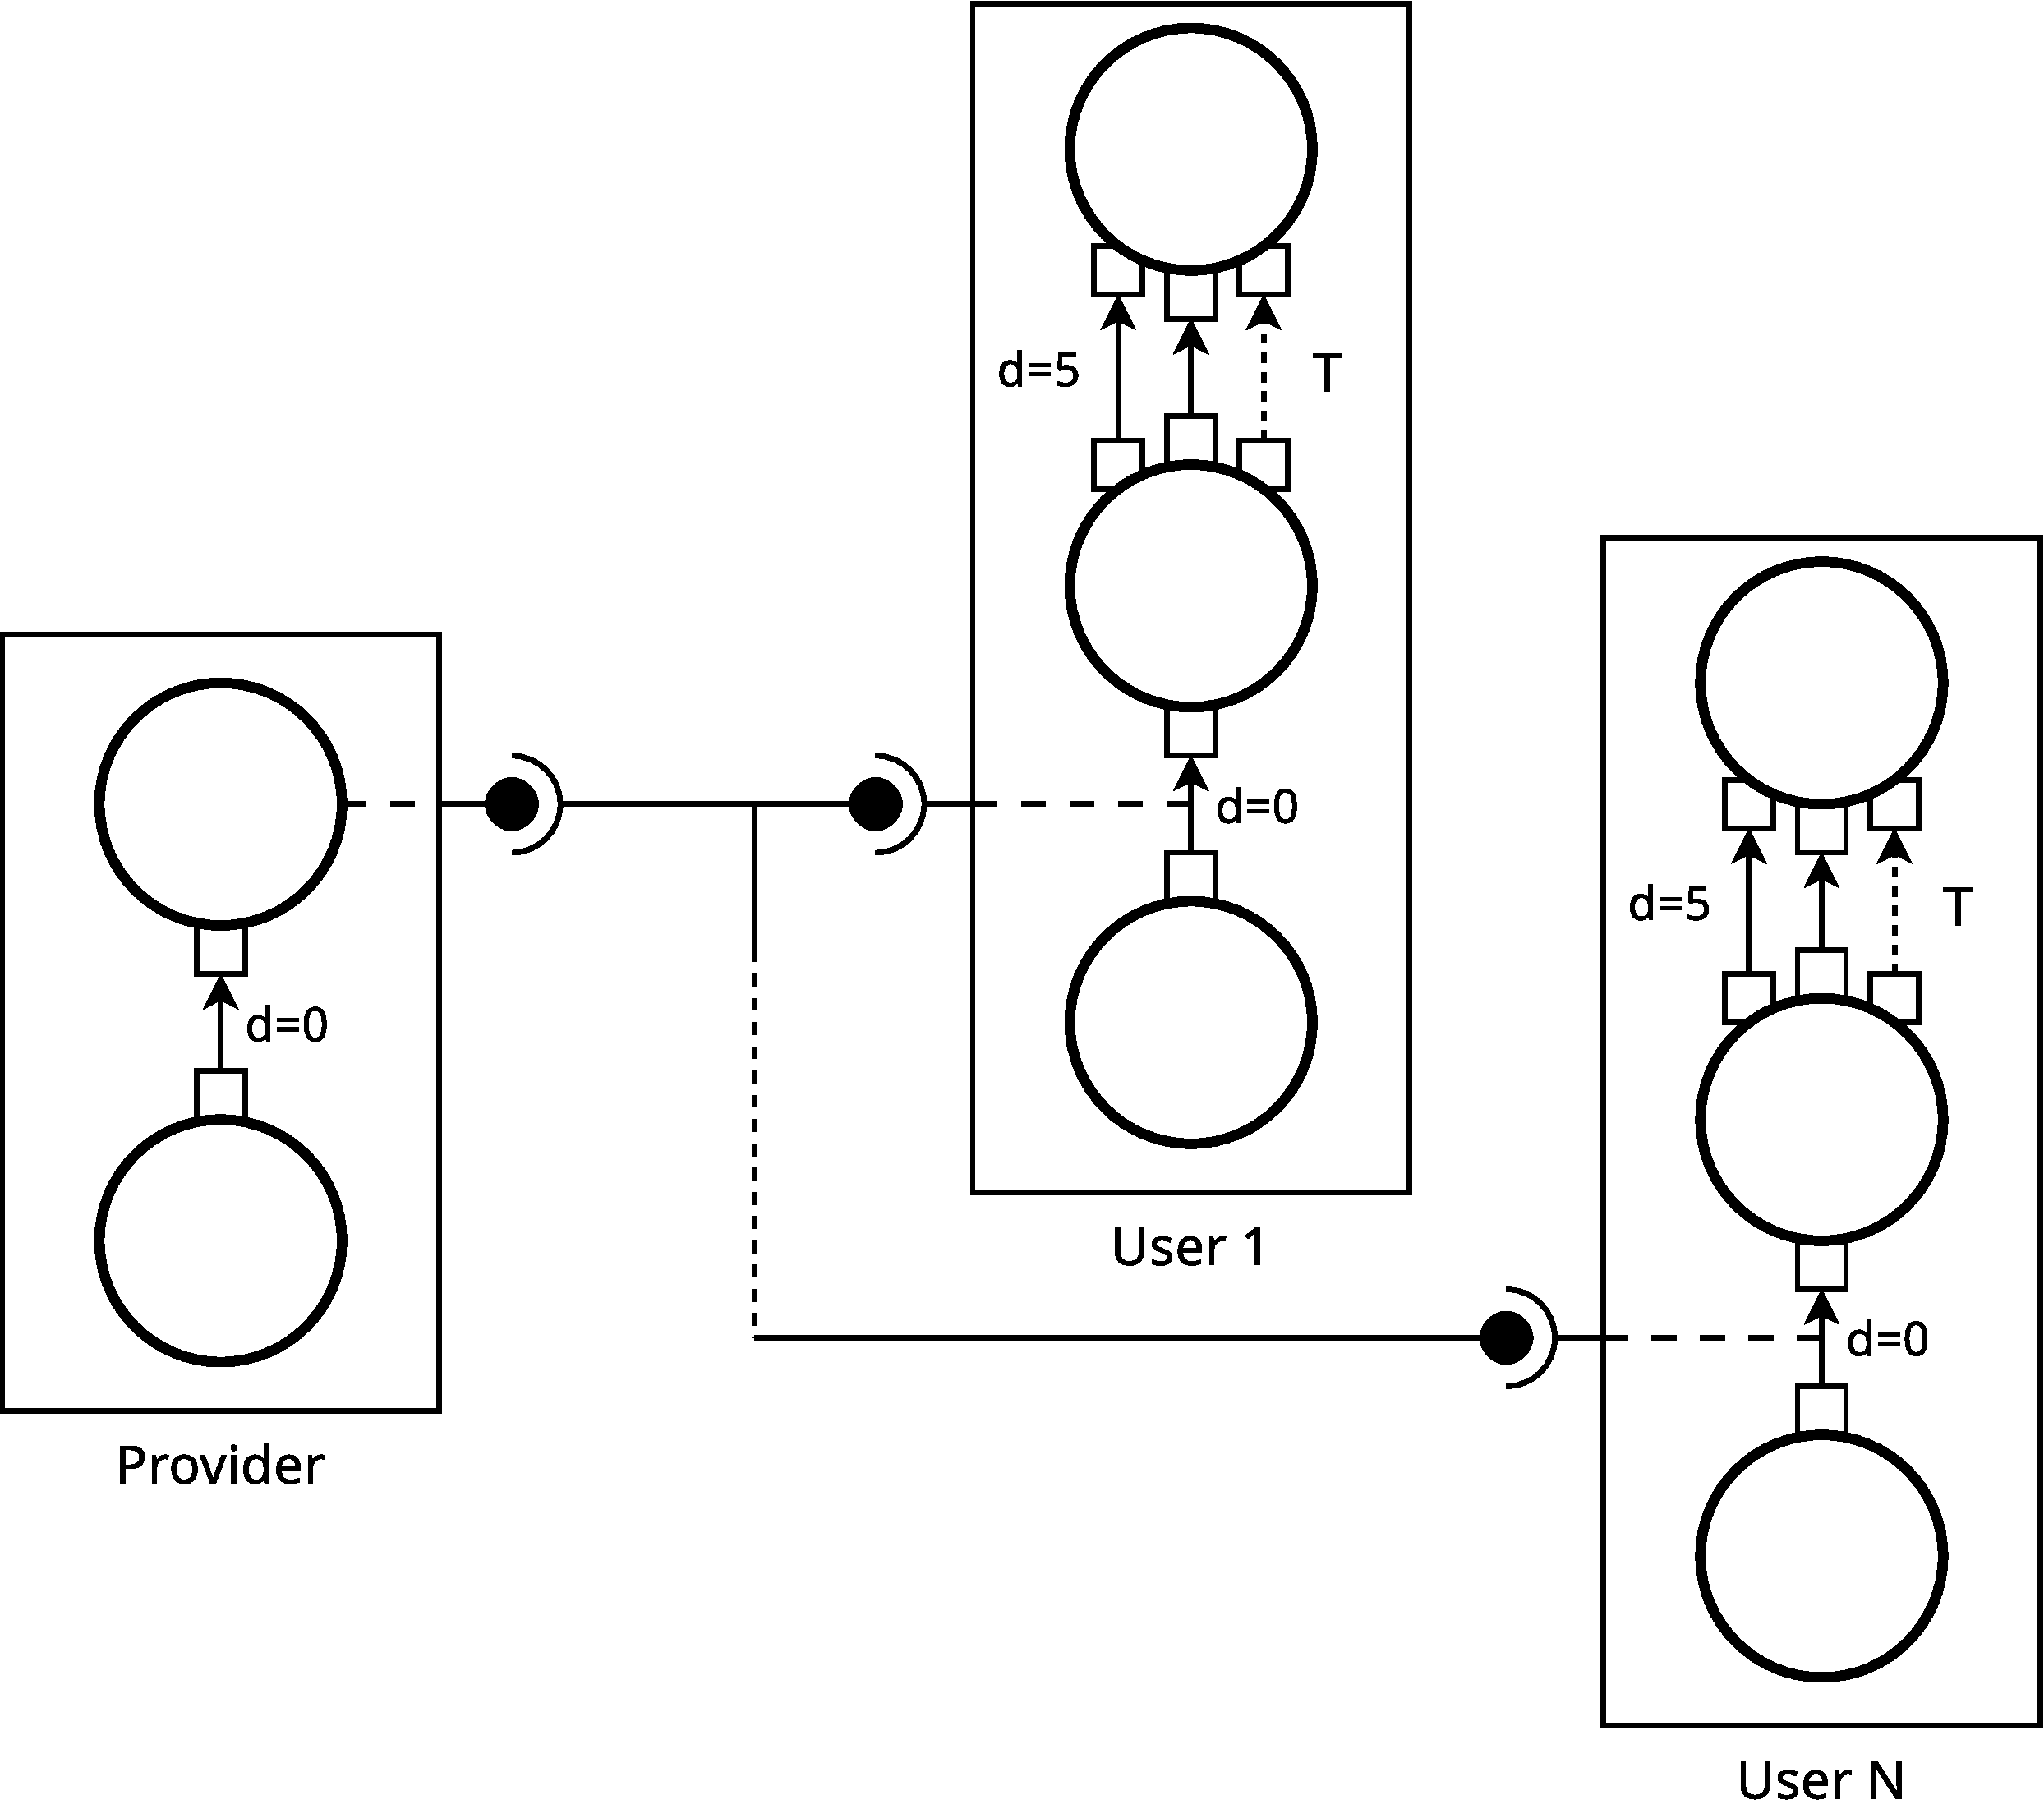
\includegraphics[width=0.4\textwidth]{./images/par.pdf}
    \caption{The parallel assembly for the Madeus benchmark, with N parallel components, and T parallel transitions.}
    \label{fig:par}
  \end{center}
\end{figure}

The second version of this assembly features a transition that calls an ssh connection and waits for a fixed amount of time, similar as for the dry-run version, before finishing. 

Two other benchmarks made with parallel assemblies written in Madeus, as depicted in Figure~\ref{fig:par}.
Their aim is to illustrate the performances of Madeus regardless of the components and the content of their transitions.

The first assembly evaluates the parallelism at the component level, when components are deployed simultaneously and the second one evaluates the parallelism at the transition level, when transitions are performed simultaneously.
The second and third benchmarks are made to evaluate the performances with parallelism both at the component level and at the transition level.

They use the same assembly that is composed of an initial \emph{provider} component and \emph{N parallel components} connected to the provider. Each component contains a first transition that uses the service provided by the provider component and \emph{T parallel transitions}. For the benchmark about component level parallelism, the number of components varies from 1 to 40 components and a fixed 1 transition, while for the benchmark about transition level parallelism, thoe number of transitions varies from 1 to 20 %link to pictures

Each benchmark was run for ten iterations with a sleep time value of 5 seconds to have a coherent scale of results.

% Parallel no ssh part

% Parallel SSH part

% Synthetic Benchmark description

%Results

\begin{figure}[h]
  \begin{center} 
    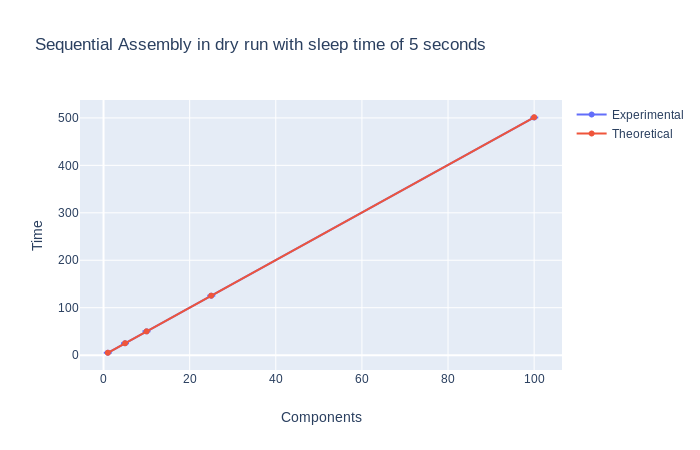
\includegraphics[width=0.5\textwidth]{./images/evaluations_dryrun_seq.png}
    \caption{Results of the sequential benchmark on dryrun}
    \label{fig:dryrunseq}
  \end{center}
\end{figure}

\begin{figure}[h]
  \begin{center} 
    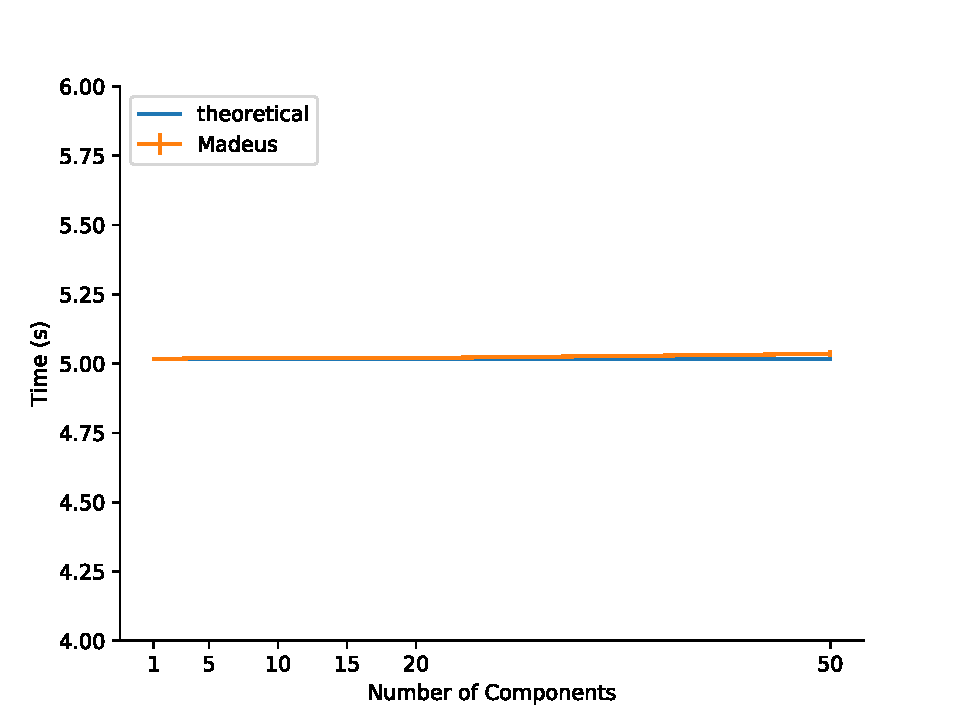
\includegraphics[width=0.5\textwidth]{./images/evaluations_par_component.pdf}
    \caption{Results of the parallel assembly benchmark with varying component number}
    \label{fig:dryrunseq}
  \end{center}
\end{figure}
\begin{figure}[h]
  \begin{center} 
    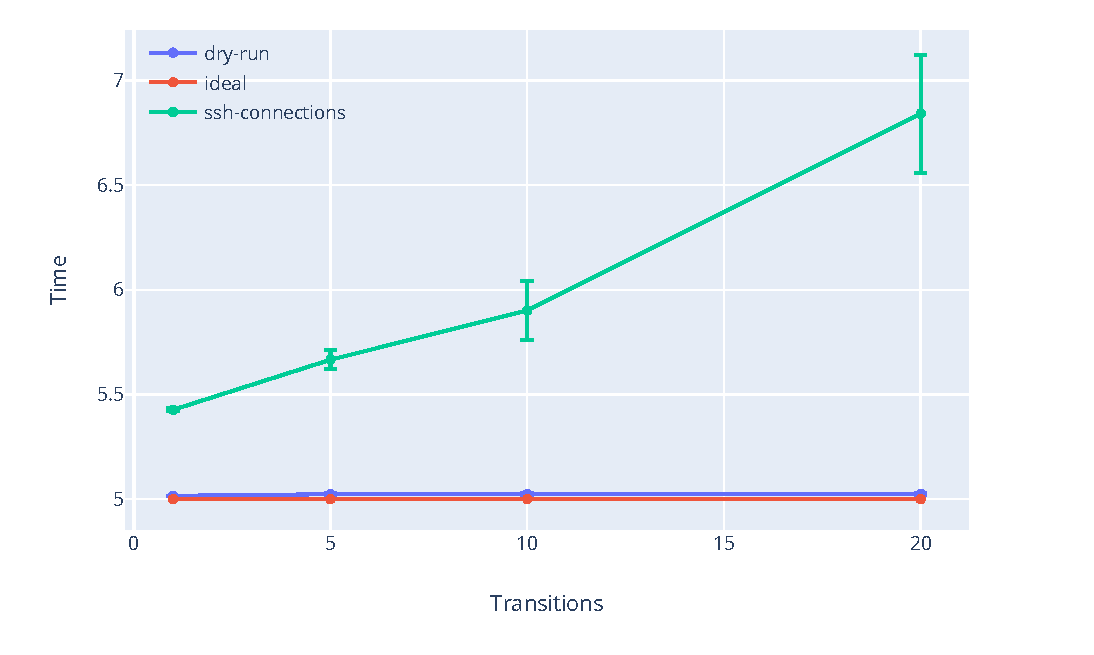
\includegraphics[width=0.5\textwidth]{./images/evaluations_par_transitions.pdf}
    \caption{Results of the parallel assembly benchmark with varying parallel transition number}
    \label{fig:dryrunseq}
  \end{center}
\end{figure}

This all helps us see that the overhead from the ssh connections is important.
\subsection{Performance model precision}

\HC[All]{a voir}

